\chapter{Lecture 1: ....}\label{lec:1}
% -------------------------------------------------------
\section{What is a System?}

A \textbf{system} is defined as a group of interacting elements that work together
as a unified whole. A car is a good example: the engine, brakes, sensors, and
software all interact, yet together they form one coherent system.

Every system has three fundamental properties:

\begin{itemize}[leftmargin=1.5em]
    \item \textbf{Structure} -- what the system is made of: its components and
    how they are connected. Examples include sensors, controllers, and networks.

    \item \textbf{Behavior} -- what the system does: it takes inputs, processes
    them, and produces outputs. These outputs could be data, energy, or physical
    actions.

    \item \textbf{Interconnectivity} -- the parts do not merely coexist; they
    have real functional relationships. The output of one component becomes the
    input of another.
\end{itemize}

% -------------------------------------------------------
\section{System Boundaries}

Before analyzing or designing a system, you must decide \textbf{where the system
ends and the outside world begins}. This is called defining the \emph{boundary}.

\begin{mdframed}[backgroundcolor=lightgray, linewidth=0pt, innertopmargin=8pt,
innerbottommargin=8pt]
\textbf{Example:} When studying a wind farm control system, do you include the
electricity market? Customer behavior? Weather? You must make a deliberate
choice. What is \emph{inside} the boundary is modelled carefully; what is
\emph{outside} is treated as a given input.
\end{mdframed}

\vspace{0.5em}
Getting boundaries right matters:
\begin{itemize}[leftmargin=1.5em]
    \item Drawing the boundary \textit{too narrowly} means missing important
    influences.
    \item Drawing it \textit{too widely} makes the problem unmanageable.
\end{itemize}

% -------------------------------------------------------
\section{System of Systems (SoS)}

A \textbf{System of Systems} is a system whose components are themselves
complete, independent systems. Each subsystem serves its own individual purpose
but also participates in the larger whole.

The key reference is Maier (1998), who identifies five characteristics that
distinguish a true SoS from merely a complicated system.

% --- characteristic boxes ---
\subsection{1. Operational Independence}

\begin{mdframed}[backgroundcolor=lightgray, linewidth=0pt, innertopmargin=6pt,
innerbottommargin=6pt]
\textbf{Plain English:} Each subsystem can survive on its own if disconnected
from the rest.
\end{mdframed}

If you pull one subsystem out, it can still do its job. Think of a wind turbine
with its local controller: even if the central controller goes offline, the
turbine can keep running using the last set-point it received. The subsystem was
designed to be useful on its own, not only as part of the larger system.

\subsection{2. Managerial Independence}

\begin{mdframed}[backgroundcolor=lightgray, linewidth=0pt, innertopmargin=6pt,
innerbottommargin=6pt]
\textbf{Plain English:} The subsystems are not just \emph{able} to run
independently -- they actually \emph{do}. Different teams or organisations own
and operate them.
\end{mdframed}

The subsystems are separately acquired, funded, and maintained. They have
their own management structures and would continue to exist even if the
System of Systems were dissolved. This is what separates a true SoS from, say,
a single company's tightly integrated product.

\subsection{3. Evolutionary Development}

\begin{mdframed}[backgroundcolor=lightgray, linewidth=0pt, innertopmargin=6pt,
innerbottommargin=6pt]
\textbf{Plain English:} The system is never truly ``finished.'' It grows and
changes over time as new parts are added or old ones are replaced.
\end{mdframed}

The system is not designed once and deployed forever. New subsystems get added,
capabilities get removed, and the overall purpose can shift. This makes SoS
design fundamentally different from designing a single product with a fixed
specification.

\subsection{4. Emergent Behavior}

\begin{mdframed}[backgroundcolor=lightgray, linewidth=0pt, innertopmargin=6pt,
innerbottommargin=6pt]
\textbf{Plain English:} The whole system can do things that \emph{none} of the
individual parts could do alone -- but it can also behave in unexpected ways
that nobody planned for.
\end{mdframed}

This is arguably the most important characteristic. Emergent behavior arises
from the \emph{interaction} between subsystems, not from any single one. For
example, a wind farm as a whole can balance and optimise power output across
turbines -- something no single turbine can do by itself. However, emergence
also introduces risk: unexpected and undesired behaviors can arise that are
difficult to predict or trace back to any one component.

\subsection{5. Geographical Distribution}

\begin{mdframed}[backgroundcolor=lightgray, linewidth=0pt, innertopmargin=6pt,
innerbottommargin=6pt]
\textbf{Plain English:} The parts are physically spread out. Because of this,
they can only share \emph{information} -- they cannot hand physical things to
each other. This is why networks are essential.
\end{mdframed}

The component systems are spread across large geographic areas. Communication
is therefore limited to data exchange, which introduces delays, potential
losses, and bandwidth constraints. This is precisely why the study of
\emph{networks} is inseparable from the study of these systems.

\vspace{1em}
Some researchers also add: \textbf{interdisciplinarity}, \textbf{heterogeneity
of components}, and \textbf{networks of systems} as further distinguishing
characteristics.

% -------------------------------------------------------
\section{Example: Wind Farm Controller}

\subsection{Setup}

A central controller manages many wind turbines spread across a geographic area.
It has two main targets:
\begin{itemize}[leftmargin=1.5em]
    \item Achieve a reference power generation level.
    \item Reduce fatigue (accumulated mechanical damage) across the turbines.
\end{itemize}

\subsection{Communication Architecture}

There are two distinct networks in the system:

\begin{itemize}[leftmargin=1.5em]
    \item \textbf{Access Network} (fiber optics, LTE, 3G, 2G, PLC) -- carries
    control set-points \emph{downward} from the central controller to each
    turbine's local controller.

    \item \textbf{Sensor Network} (Fieldbus, CANbus, WSN) -- carries sensor
    measurements \emph{upward} from 3 sensors per turbine (2 torque sensors,
    1 rotation angle sensor) through a gateway to the central controller.
\end{itemize}

\subsection{The Network Impact: Timing and Offsets}

This is the core insight of the example. Sensors send measurements
periodically, and there is a configurable \emph{offset} $T_o$ -- the delay
between $t=0$ and when the sensor actually transmits. The key parameters are:

\begin{center}
\begin{tabular}{lll}
\toprule
\textbf{Parameter} & \textbf{Symbol} & \textbf{Value} \\
\midrule
Control period      & $T_s$       & 150 ms \\
Computation time    & $T_{compute}$& 50 ms  \\
Configurable offset & $T_o$       & variable \\
\bottomrule
\end{tabular}
\end{center}

There is an inherent trade-off:

\begin{itemize}[leftmargin=1.5em]
    \item \textbf{Too small} $T_o$: the sensor data has not yet arrived when
    the controller needs to compute. The computation uses stale or missing data.

    \item \textbf{Too large} $T_o$: the data \emph{is} available, but it
    describes the turbine's state from too far in the past -- the information
    has ``aged.''
\end{itemize}

Experiments show accumulated damage decreases as $T_o$ increases up to
$T_o = 100$\,ms, then rises again. Beyond 100\,ms, the turbine has already
received the \emph{previous} control set-point, so the sensor samples a system
operating under an outdated command -- degrading control performance.

\begin{mdframed}[backgroundcolor=lightgray, linewidth=0pt, innertopmargin=8pt,
innerbottommargin=8pt]
\textbf{Key Takeaway:} Network behavior is not merely an IT concern. Delays,
timing, and reliability in the communication network \emph{directly} affect the
physical performance of the controlled system. This motivation underpins the
entire Networks and Systems course.
\end{mdframed}

\clearpage
\section*{The OSI Model --- Why It Exists}

Before talking about network performance, the lecturer establishes a common language using the OSI layer model.

The idea is simple: networking is complex, so engineers broke it into 7 layers, where each layer has a specific job and only talks to the layers directly above and below it.

Think of it like sending a letter internationally --- you write it, put it in an envelope, address it, hand it to a postal service, it gets loaded on a truck, then a plane, then another truck. Each ``layer'' of that process has its own rules and doesn't need to know the details of the others.

The layers from bottom to top are:

\subsection*{Layer 1 --- Physical}

Raw transmission of bits over a medium. Cables, radio waves, light pulses. It deals in symbols.

\subsection*{Layer 2 --- Link Layer}

Layer 2 only cares about one single hop --- getting data from one device to the next directly connected device. It has absolutely no concept of anything beyond that immediate neighbour.

This is where MAC addresses live. A MAC address identifies a network interface on the local network, like:

\begin{verbatim}
00:1A:2B:3C:4D:5E
\end{verbatim}

Switches mainly operate at Layer 2. They forward frames between devices inside the same local network (LAN).

The important thing is that MAC addresses are only meaningful locally. Your laptop does not know Google's MAC address --- it only knows the MAC address of the next device it must talk to, usually your router.

Layer 2 also handles:
\begin{itemize}
    \item Framing
    \item Error checking (CRC)
    \item Medium access control (who gets to transmit)
\end{itemize}

\subsection*{Layer 3 --- Network Layer}

Layer 3 is where end-to-end routing happens. It knows the full journey from source to destination and figures out which path to take across potentially many hops and many different networks.

This is where IP lives.

Examples:
\begin{itemize}
    \item \texttt{192.168.1.5}
    \item \texttt{8.8.8.8}
\end{itemize}

Routers operate here.

While Layer 2 only thinks:

\begin{quote}
``Which directly connected neighbour gets this frame?''
\end{quote}

Layer 3 thinks:

\begin{quote}
``How do I reach that destination across the internet?''
\end{quote}

A packet may travel through many routers before reaching its final destination. Each router examines the destination IP address and decides where to forward the packet next.

So:
\begin{itemize}
    \item Layer 2 = local delivery between neighbours
    \item Layer 3 = global routing across networks
\end{itemize}

\subsection*{Layer 4 --- Transport Layer}

Layer 3 got the packet to the right building (computer). Layer 4's job is to get the data to the right apartment (application) inside that building, and to manage the reliability of the delivery.

This is where TCP and UDP live.

Layer 4 uses port numbers to identify applications:
\begin{itemize}
    \item Port 80 $\rightarrow$ HTTP
    \item Port 443 $\rightarrow$ HTTPS
    \item Port 22 $\rightarrow$ SSH
\end{itemize}

\subsubsection*{TCP}

TCP is reliable.

It:
\begin{itemize}
    \item Checks if packets arrived
    \item Retransmits lost packets
    \item Keeps packets in order
    \item Performs flow and congestion control
\end{itemize}

Used for things like:
\begin{itemize}
    \item Web browsing
    \item File downloads
    \item SSH
\end{itemize}

Reliability matters more than speed.

\subsubsection*{UDP}

UDP is lightweight and fast.

It:
\begin{itemize}
    \item Sends packets without guarantees
    \item Does not retransmit lost packets
    \item Does not enforce ordering
\end{itemize}

Used for:
\begin{itemize}
    \item Voice calls
    \item Gaming
    \item Video streaming
    \item DNS queries
\end{itemize}

Low latency matters more than perfect reliability.

\subsection*{Layers 5, 6, 7 --- Session, Presentation, Application}

Higher-level concerns like:
\begin{itemize}
    \item Session management (cookies, tokens)
    \item Data representation (HTML, JSON, audio/video codecs)
    \item Actual applications and protocols (HTTP, FTP, SSH, VoIP)
\end{itemize}

The lecturer also makes an important practical note: cellular networks (4G, 5G) are extremely complex internally and have their own layered systems, but from the outside you can mostly treat them as another Layer 1/2 access technology feeding into an IP network.

% -------------------------------------------------------
\section{Performance Metrics Per Layer}
\todo{Make sure to look back at this again and remember most}
This is where the OSI model becomes practically useful. Each layer has its own
data unit and its own performance metrics. Different layers therefore measure
different aspects of network behavior.

\subsection{Layer 1 --- Symbol Level}

At the Physical Layer, the focus is on transmitting raw symbols over the
physical medium.

Important metrics are:
\begin{itemize}[leftmargin=1.5em]
    \item Symbol transmission duration
    \item Symbol decoding success probability
\end{itemize}

This layer only concerns whether the receiver can correctly interpret the
electrical, optical, or radio signal being transmitted.

\subsection{Layer 2 --- Frame Level}

At Layer 2, bits are grouped into \emph{frames} and transferred between directly
connected devices.

Key metrics include:
\begin{itemize}[leftmargin=1.5em]
    \item Frame delay (one-way or round-trip)
    \item Frame transmission success probability
    \item Layer 2 throughput
    \item Layer 2 goodput
\end{itemize}

Because Layer 2 only operates locally, these metrics describe performance across
a \emph{single hop}.

\subsection{Layer 3 --- Packet Level}

Layer 3 deals with IP packets moving across potentially many routers and
networks.

Important metrics are:
\begin{itemize}[leftmargin=1.5em]
    \item End-to-end IP packet delay
    \item Packet delivery probability
    \item Packet loss probability
    \item Layer 3 throughput
    \item Layer 3 goodput
\end{itemize}

Packet delivery probability is simply:

\[
P_{\text{delivery}} = 1 - P_{\text{loss}}
\]

Unlike Layer 2, these metrics describe the \emph{entire path} between source
and destination.

\subsection{Layer 4 --- Segment Level (TCP/UDP)}

Layer 4 focuses on communication between applications running on end hosts.

Metrics include:
\begin{itemize}[leftmargin=1.5em]
    \item End-to-end delay
    \item Round-trip time (RTT)
    \item Layer 4 throughput
    \item Layer 4 goodput
\end{itemize}

TCP introduces additional performance considerations because it handles:
\begin{itemize}[leftmargin=1.5em]
    \item Reliability
    \item Retransmissions
    \item Flow control
    \item Congestion control
\end{itemize}

UDP, by contrast, minimizes overhead and delay by avoiding reliability
mechanisms.

\subsection{Application Layer}

At the Application Layer, performance metrics become application-specific.

In the wind farm example, the important metrics were:
\begin{itemize}[leftmargin=1.5em]
    \item Reference tracking accuracy
    \item Accumulated mechanical damage
\end{itemize}

The lower-layer network metrics directly influence these higher-level system
outcomes.

% -------------------------------------------------------
\section{Throughput vs Goodput}

This distinction is extremely important.

\begin{mdframed}[backgroundcolor=lightgray, linewidth=0pt,
innertopmargin=8pt, innerbottommargin=8pt]
\textbf{Throughput} measures all transmitted bits per second, including:
\begin{itemize}
    \item Protocol headers
    \item Control information
    \item Retransmissions
\end{itemize}

\textbf{Goodput} measures only the useful application payload bits delivered
per second.
\end{mdframed}

Goodput is therefore always less than or equal to throughput:

\[
\text{Goodput} \leq \text{Throughput}
\]

In practice, goodput is usually what matters most to the application.

% -------------------------------------------------------
\section{The 2-Hop Network Setting}

To make the discussion concrete, the lecturer introduces a simple network:

\begin{center}
Host A $\rightarrow$ Router $\rightarrow$ Host B
\end{center}

The two links may use completely different technologies:
\begin{itemize}[leftmargin=1.5em]
    \item Ethernet on one side
    \item Cellular (4G/5G) on the other
\end{itemize}

This setup illustrates an important systems insight:

\begin{mdframed}[backgroundcolor=lightgray, linewidth=0pt,
innertopmargin=8pt, innerbottommargin=8pt]
End-to-end performance is not determined by a single link. Delay, loss, and
throughput emerge from the combined behavior of all links, routers, queues, and
technologies along the path.
\end{mdframed}

Even a very fast link can still produce poor end-to-end performance if another
hop becomes congested or unreliable.

% -------------------------------------------------------
\section{Sources of Delay}

The lecturer breaks end-to-end delay into several components. This is one of
the most exam-relevant parts of the lecture.

\subsection{Delays at the Sending Host}

Before data even leaves the sender, several delays may occur:

\begin{itemize}[leftmargin=1.5em]
    \item \textbf{Processing and accumulation at Layer 4} \\
    TCP may need time to build a segment before transmission.

    \item \textbf{Connection setup} \\
    TCP requires a handshake before communication begins.

    \item \textbf{DNS lookup} \\
    A hostname may first need to be translated into an IP address.

    \item \textbf{Output queueing} \\
    Packets may wait in Layer 3/2 queues before transmission.

    \item \textbf{Medium access delay} \\
    The sender may need permission to use the medium (especially in wireless systems).

    \item \textbf{Serialization delay} \\
    The time required to place all bits onto the wire.

    \item \textbf{Retransmissions} \\
    Failed frames or segments may need to be resent.
\end{itemize}

\subsection{Delays at the Router}

Routers introduce additional delay sources:

\begin{itemize}[leftmargin=1.5em]
    \item Packet header processing
    \item Routing decisions
    \item Input and output queueing
    \item Route discovery (in dynamic routing systems)
    \item Medium access on the outgoing link
    \item Serialization on the outgoing link
    \item Possible retransmissions
\end{itemize}

\subsection{Propagation Delay}

Propagation delay is fundamentally different from the previous delays.

It is the time required for the physical signal to travel through space or
through the transmission medium.

Propagation delay depends on:
\begin{itemize}[leftmargin=1.5em]
    \item Distance
    \item Signal propagation speed
\end{itemize}

Importantly, it does \emph{not} depend on the data rate.

\subsection{Key Insight: Different Delays Depend on Different Things}

Different delay components arise from completely different mechanisms:

\begin{itemize}[leftmargin=1.5em]
    \item \textbf{Serialization delay} depends on packet size and transmission rate.

    \item \textbf{Propagation delay} depends on physical distance.

    \item \textbf{Queueing delay} depends on network load and congestion.
\end{itemize}

Queueing delay is especially important because it is \emph{stochastic} --- it
varies randomly over time depending on traffic conditions.

This is why probabilistic and queueing models become essential in network
analysis.

% -------------------------------------------------------
\section{Sources of Packet Loss see slide 27}

Packet loss can occur at several layers for different reasons.

\subsection{Layer 1 Losses}

At the Physical Layer, the receiver may fail to decode the signal correctly.

Reasons include:
\begin{itemize}[leftmargin=1.5em]
    \item Weak signal strength
    \item Noise
    \item Interference
\end{itemize}

\subsection{Layer 2 Losses}

At Layer 2, frames may be dropped because of:

\begin{itemize}[leftmargin=1.5em]
    \item Collisions
    \item CRC/checksum mismatch
    \item Buffer overflow
\end{itemize}

A checksum failure means the receiver detected corruption in the frame.

\subsection{Layer 3 Losses}

At Layer 3, packets may be lost because:
\begin{itemize}[leftmargin=1.5em]
    \item No route exists to the destination
    \item Router buffers overflow
\end{itemize}

Congested routers commonly drop packets when queues become full.

\subsection{Layer 4 and Above}

Higher-layer losses can also occur:
\begin{itemize}[leftmargin=1.5em]
    \item TCP checksum failure
    \item Session drops
    \item Application decoding errors
\end{itemize}

% -------------------------------------------------------
\section{Compounding Packet Loss Across Hops}

A very important insight is that packet loss compounds across multiple hops.

If each link has a delivery probability $P_i$, then the overall end-to-end
delivery probability becomes:

\[
P_{\text{end-to-end}} = \prod_{i=1}^{N} P_i
\]

Equivalently, small packet loss probabilities accumulate across the network.

This means even highly reliable individual links can still produce noticeable
end-to-end loss when many hops are involved.

\clearpage

\section*{What Does ``Continuous'' Mean Continuous Time Markov chains (CTMC)s?}

``Continuous'' refers to \textbf{time} being a continuous variable (\(t \in \mathbb{R}_{\ge 0}\)), not to the state space. 
The state space itself can be discrete (finite or countably infinite). 
Thus, a CTMC is a stochastic process \(\{X_t, t \ge 0\}\) where:
\begin{itemize}
    \item \(t\) evolves continuously (not in steps like discrete-time Markov chains).
    \item \(X_t\) takes values in a discrete set \(\mathbb{E}\) (the state space).
    \item Transitions between states occur at random times, and the holding times are exponential.
\end{itemize}
\vspace{0.3cm}
\begin{mdframed}[backgroundcolor=lightgray, linewidth=0pt, innertopmargin=8pt,
innerbottommargin=8pt]
\textbf{Key Takeaway:} in a continuous-time Markov chain (CTMC), transitions can happen at any real time – not just at fixed, discrete time steps (like t = 1, 2, 3, … seconds).
\end{mdframed}
\section*{Core Concepts of Continuous Time Markov chains (CTMCs}

\begin{table}[h!]
\centering
\begin{tabular}{>{\raggedright\arraybackslash}p{3.5cm} 
                >{\raggedright\arraybackslash}p{7cm} 
                >{\raggedright\arraybackslash}p{4cm}}
\toprule
\textbf{Concept} & \textbf{What it means} & \textbf{Mathematical notation} \\
\midrule
State space & The set of all possible states the system can be in. Can be finite (e.g., \(0,1,2,\dots,K\)) or infinite (\(0,1,2,\dots\)). & \(\mathbb{E} = \{0,1,2,\dots\}\) or \(\{0,1,\dots,K\}\) \\
\hline
Transition rate & How fast the system moves from state \(j\) to state \(k\) (average number of transitions per unit time). & \(\mu_{jk}\) \\
\hline
Total rate out of state \(j\) & Sum of all rates leaving state \(j\). & \(\mu_j = \sum_{k \neq j} \mu_{jk}\) \\
\hline
Transition probability & Given we leave state \(j\), the chance we go to state \(k\). & \(\dfrac{\mu_{jk}}{\mu_j}\) \\
\hline
State random variable & The state of the system at time \(t\) – it is random. & \(X_t\) \\
\hline
State probability & Probability that the system is in state \(i\) at time \(t\). & \(\pi_i(t) = \Pr(X_t = i)\) \\
\hline
Markov property & Future depends only on current state, not on history. & \(\Pr(X_{t_n}=j \mid \text{past}) = \Pr(X_{t_n}=j \mid X_{t_{n-1}}=i)\) \\
\hline
Chapman-Kolmogorov equation & How state probabilities change over time (rate of change = inflow \(-\) outflow). & \(\dfrac{d\pi_i(t)}{dt} = -\mu_i \pi_i(t) + \sum_{j \neq i} \mu_{ji} \pi_j(t)\) \\
\hline
Steady-state flow balance & In equilibrium: total flow out of state \(i\) equals total flow into state \(i\). & \(\mu_i \pi_i = \sum_{j \neq i} \mu_{ji} \pi_j\) \\
\bottomrule
\end{tabular}
\caption{Definitions and notation for continuous-time Markov chains}
\end{table}

\noindent
These equations form the foundation for analyzing buffering and multiplexing in network nodes (Layer 2 and Layer 3 performance).


\section{Why Exponential Holding Times?}
\todo{skal lige forstå hvorfor det er exponetial}
In a \textbf{continuous-time Markov chain (CTMC)}, the time spent in any state (the \textit{holding time}) must be exponentially distributed. 
The reason is the \textbf{memoryless property}:
\[
\Pr(T > t + s \mid T > s) = \Pr(T > t)
\]
This property ensures that the future evolution depends only on the current state, not on how long the system has already been in that state. 
Without exponential holding times, the Markov property would not hold in continuous time. 
Exponential distributions also make the mathematics tractable: they lead to linear differential equations (Chapman-Kolmogorov) and closed-form steady-state solutions (e.g., M/M/1 queue, Erlang-B formula).

\section{What is Kendall Notation?}

It is a shorthand to describe a queueing system.
The basic form is: 
\[
\mathbf{X / Y / C / B}
\]

\begin{table}[h!]
\centering
\caption{Kendall notation fields}
\begin{tabular}{>{\raggedright\arraybackslash}p{2.5cm} 
                >{\raggedright\arraybackslash}p{2.5cm} 
                >{\raggedright\arraybackslash}p{3.5cm} 
                >{\raggedright\arraybackslash}p{6cm}}
\toprule
\textbf{Field} & \textbf{Name} & \textbf{Possible values} & \textbf{Meaning} \\
\midrule
X & Arrival process & M, GI, G & Distribution of time between arrivals \\
\hline
Y & Service process & M, G, D & Distribution of service time \\
\hline
C & Servers & 1,2,3,\dots & How many packets served simultaneously \\
\hline
B & Buffer size & integer or \(\infty\) & Max packets in system (if finite, packets can be lost) \\
\hline
(optional) & Discipline & FIFO, PS, LIFO, EDF & Order of serving waiting packets \\
\bottomrule
\end{tabular}
\end{table}

\noindent
\textbf{Note:} Sometimes you see X/Y/C (no B) meaning infinite buffer.
Sometimes X/Y/C/B with B including the one in service.

\section*{Detailed breakdown of each field}

\subsection*{1. X = Arrival process}

Describes the \textbf{time between arrivals} (inter-arrival times).

\begin{itemize}
    \item \textbf{M} = Markovian (memoryless) \(\rightarrow\) inter-arrival times are exponentially distributed \(\rightarrow\) the arrival process is a \textbf{Poisson process} (arrivals happen at any time, independently).
    \item \textbf{GI} = General Independent \(\rightarrow\) inter-arrival times are independent and identically distributed (iid) but can follow any distribution (e.g., uniform, deterministic, Pareto). No memoryless property assumed.
    \item \textbf{G} = General (may not even be iid, but usually we assume iid in basic models).
\end{itemize}

\subsection*{2. Y = Service process}

Describes the \textbf{time to serve one packet} (service time).

\begin{itemize}
    \item \textbf{M} = Markovian \(\rightarrow\) exponentially distributed service times.
    \item \textbf{G} or \textbf{GI} = General distribution (e.g., constant, uniform, heavy-tailed).
    \item \textbf{D} = Deterministic (constant service time).
\end{itemize}

\subsection*{Service discipline (not always in Kendall notation, but important)}

Besides X/Y/C/B, you often need to specify \textbf{which packet is served next} when multiple are waiting.

\begin{itemize}
    \item \textbf{FIFO} (First-In-First-Out) = default, like a queue at a supermarket.
    \item \textbf{Processor Sharing (PS)} = all active packets get a tiny fraction of the server (e.g., round‑robin with very small time slices).
    \item \textbf{LIFO} (Last-In-First-Out) = last arrived gets served first. Can be preemptive (interrupts current service) or non‑preemptive.
    \item \textbf{EDF} (Earliest Deadline First) = packet with closest deadline goes next (used in real‑time systems).
\end{itemize}

\section{M/M/1 Queue in Kendall Notation}
\begin{figure}[H]
    \centering
    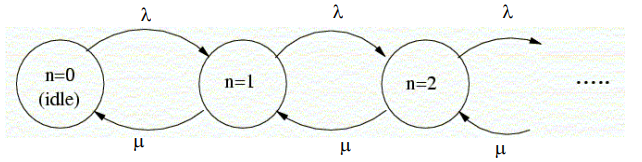
\includegraphics[width=0.8\linewidth]{figures/Lecture1/mm1queue.png}
    \label{fig:placeholder}
\end{figure}
The M/M/1 queue is described by the Kendall notation:
\[
\mathbf{M / M / 1}
\]
which means:
\begin{itemize}
    \item \textbf{First M}: Poisson arrival process (Markovian) with rate \(\lambda\) (exponentially distributed inter-arrival times).
    \item \textbf{Second M}: Exponentially distributed service times with rate \(\mu\).
    \item \textbf{1}: Single server.
    \item \textbf{Non 4th parameter:} means indefinite queue buffer
    \item \textbf{Service discipline}: FIFO (First-In-First-Out) by default.
\end{itemize}

\subsection*{System Dynamics}
Let \(Q_t\) be the number of packets in the system (queue + served) at time \(t\).  
Because of the memoryless (exponential) assumptions, \(\{Q_t, t \ge 0\}\) At every time \(t\) from 0 onward, the queue length is some non‑negative integer. It is a \textbf{continuous-time Markov chain} (CTMC) with state space \(\mathbb{E} = \{0,1,2,\dots\}\), where states is the total number of packets in the system (queue + served).
\begin{itemize}
    \item \(Q_t = 0\) means the server is idle (no packets).
    \item \(Q_t \ge 1\) means the server is busy, and \(Q_t - 1\) packets are waiting in the queue.
\end{itemize}
\subsection*{Utilization}
The utilization factor is defined as:
\[
\rho = \frac{\lambda}{\mu}
\]
\begin{itemize}
    \item \(\lambda\) = average arrival rate (packets per second).  
          Arrivals follow a Poisson process (exponentially distributed inter-arrival times with mean \(1/\lambda\)).
    \item \(\mu\) = average service rate (packets per second).  
          Service times are exponentially distributed with mean \(1/\mu\).  
          The server can handle at most \(\mu\) packets per second when busy.
\end{itemize}
If \(\rho \ge 1\), the system is unstable (no steady-state distribution; the queue grows indefinitely).  
For a stable system we require \(\rho < 1\).

\section{Performance Parameters M/M/1 like (Steady-State, \(\rho < 1\)), Birth-Death Process}

\begin{itemize}
    \item \textbf{Queue-length distribution}:
    \[
    \pi_i = \Pr(Q = i) = (1 - \rho) \rho^i, \quad i = 0,1,2,\dots
    \]
    Probability of i packets in queue [using flow-balance equations]

    probality of idle server
    \[
    \pi_0  = (1 - \rho)
    \]
    \item \textbf{Average queue length} (including the packet in service):
    \[
    \mathbb{E}[Q] = \frac{\rho}{1 - \rho}
    \]
    \item \textbf{Average system time} (delay from arrival to departure):
    \[
    \mathbb{E}[S] = \frac{1}{\mu - \lambda}
    \]
    \(\mu\) = average service rate (packets per second) minus, \(\lambda\) = average arrival rate (packets per second), with means of \(1/\mu\), \(1/\rho\) therefore resulting in this
    \item \textbf{Buffer overflow probability} (for a finite buffer of size \(B\)):
    By the PASTA property (Poisson Arrivals See Time Averages), an arriving packet sees the same distribution as the time-average. Thus the probability that an arriving packet finds \(B\) or more packets in the system is:
    \[
    \Pr(\text{arrival sees } Q \ge B) = \Pr(Q \ge B) = \rho^B
    \]
\end{itemize}

\noindent
\textbf{Note}: The M/M/1 model is the foundation for analyzing buffering and multiplexing in network nodes (Layer 2 and Layer 3 performance).

\section{Circuit-Switched Approach – How it works}

\begin{enumerate}[label=\textbf{Step \arabic*}:]
    \item \textbf{Call setup phase} – the network finds an end‑to‑end path and reserves resources (e.g., one physical channel, a fixed bandwidth).
    \item \textbf{Data transfer} – the reserved resources are used exclusively by that call.
    \item \textbf{Teardown} – when the call ends, resources are released.
\end{enumerate}

\subsection*{Advantage}
Guaranteed quality (no queueing delays, no jitter, no loss due to congestion).

\subsection*{Disadvantage}
Inefficient for bursty traffic – even when you say nothing, the channel stays idle but cannot be used by others.

\subsection*{Examples}
\begin{itemize}
    \item Traditional telephone networks (POTS)
    \item ISDN (Integrated Services Digital Network)
    \item 2G mobile networks before GPRS (e.g., GSM circuit-switched calls)
\end{itemize}

\bigskip

\section{Packet-Switched Approach – How it works}

\begin{enumerate}[label=\textbf{Step \arabic*}:]
    \item No reservation. Packets are sent as soon as they are generated.
    \item Routers \textbf{store and forward} packets. If many packets arrive at the same time, they are placed in a buffer (queue) and sent one after another.
\end{enumerate}

\subsection*{Advantages}
\begin{itemize}
    \item \textbf{Flexibility} – the network adapts to varying traffic loads automatically.
    \item \textbf{Optimal resource usage} – idle periods of one user are filled with packets from other users \(\rightarrow\) \textbf{multiplexing gain}.
    \item Especially good for \textbf{bursty applications} like web browsing, sensor data access (where data comes in short bursts, not continuously).
\end{itemize}

\subsection*{Drawbacks}
\begin{itemize}
    \item Buffering/queueing at routers \(\rightarrow\) can cause:
    \begin{itemize}
        \item \textbf{Delay} (packets wait in line)
        \item \textbf{Jitter} (variation in delay between packets)
        \item \textbf{Packet loss} (if buffer is full, new packets are dropped)
    \end{itemize}
\end{itemize}

\subsection*{Examples}
\begin{itemize}
    \item The Internet (IP)
    \item Ethernet
    \item Wi-Fi (802.11)
    \item Modern cellular data (GPRS, 4G, 5G in packet-switched mode)
\end{itemize}

\section*{Why do we need mathematical models?}

Because of the drawbacks of packet switching, we need mathematical models (like Markov chains, M/M/1 queues, birth-death processes, etc.) to analyze and predict:
\begin{itemize}
    \item Average queue length
    \item Packet delay and jitter
    \item Packet loss probability
    \item Throughput
\end{itemize}
These models help network engineers design buffers, schedulers, and congestion control mechanisms.


\section{What is a Birth-Death Process?}

A birth-death process is a special type of continuous-time Markov chain where the \textbf{state} (usually the number of packets in the system) can only change by \(+1\) (birth = arrival) or \(-1\) (death = departure).

\begin{itemize}
    \item Birth rate when in state \(k\) is \(\lambda_k\) (arrival rate may depend on current number of packets).
    \item Death rate when in state \(k\) is \(\mu_k\) (service rate may depend on current number, e.g., multiple servers).
\end{itemize}

This is a generalization of the M/M/1 queue (where \(\lambda_k = \lambda\) constant, \(\mu_k = \mu\) constant for \(k \ge 1\), and \(\mu_0 = 0\) because no departure when empty).

\section{Steady-State Probabilities}

From the flow balance equations (slide 31), we can derive a product-form solution:

\[
\pi_i = \Pr(Q = i) =\pi_0 \frac{\prod_{k=0}^{i-1} \lambda_k}{\prod_{k=1}^{i} \mu_k}= \pi_0 \prod_{k=0}^{i-1} \frac{\lambda_k}{\mu_{k+1}}, \qquad i = 1,2,3,\dots
\]
\begin{mdframed}[backgroundcolor=lightgray, linewidth=0pt, innertopmargin=8pt,
innerbottommargin=8pt]
\textbf{Key Takeaway:}
The probability of being in state \(i\) is the probability of being in state 0, multiplied by the product of the ratios of birth rates to death rates as you climb from 0 up to \(i-1\).
\end{mdframed}

\section{Slide 37: Sets up the problem}

\subsection*{Scenario}
\begin{itemize}
    \item We have \(K\) channels (like \(K\) phone lines).
    \item Each call uses 1 channel for its whole duration.
    \item If all \(K\) channels are busy, a new call is \textbf{blocked} (gets a busy signal, not queued).
    \item Question: How many channels \(K\) do we need so that the blocking probability is below some target (e.g., 1\%)?
\end{itemize}

\subsection*{Assumptions (to make the problem tractable)}
\begin{itemize}
    \item Calls arrive randomly: \textbf{Poisson process} with rate \(\lambda\) (calls per second). This is realistic when many users call independently.
    \item Call duration is random: \textbf{exponentially distributed} with mean \(T\) seconds. This is okay for voice calls.
\end{itemize}

\section{Slide 38: How we model it using a Markov chain M/M/K/K}
\begin{figure}[H]
    \centering
    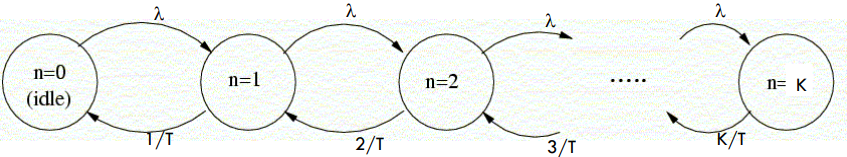
\includegraphics[width=0.8\linewidth]{figures/Lecture1/MMKK.png}
    \label{fig:placeholder}
\end{figure}

We model the \textbf{number of active calls} as a continuous-time Markov chain – specifically a \textbf{finite birth-death process} (states \(0,1,2,\dots,K\)).

\begin{itemize}
    \item \textbf{State \(i\)} = \(i\) active calls.
    \item \textbf{Birth (arrival)} from state \(i\) to \(i+1\) occurs at rate \(\lambda\) (as long as \(i < K\)). When \(i = K\), no birth (arrivals are blocked).
    \item \textbf{Death (departure)} from state \(i\) to \(i-1\) occurs at rate \(i \times (1/T)\). Why? Each of the \(i\) active calls ends at rate \(1/T\), and they are independent, so total death rate = \(i/T\).
\end{itemize}

This is an \textbf{M/M/K/K} queue in Kendall notation:
\begin{itemize}
    \item M = Markovian arrivals (Poisson)
    \item M = Markovian service (exponential)
    \item K = number of servers
    \item K = buffer size (no waiting room, so K = number of servers)
\end{itemize}

Because it is a finite birth-death process, we can solve for the steady-state probabilities using the general birth-death formula:
\[
\pi_i = \pi_0 \frac{(\lambda T)^i}{i!}, \qquad i = 0,\dots,K \qquad with \qquad \pi_0 =\frac{1}{\sum_{i=0}^{K} \frac{(\lambda T)^i}{i!}}.
\]
The \textbf{blocking probability} is simply \(\pi_K\) (the probability that all \(K\) channels are busy when a call arrives). That formula is the \textbf{Erlang-B formula}:
\[
P_{\text{block}} = \pi_K = \frac{(\lambda T)^K / K!}{\sum_{i=0}^{K} \frac{(\lambda T)^i}{i!}}.
\]

\section{M/M/1/K Queue: Performance}
\todo{maybe look at bit more at this formulas}
\begin{figure}[H]
    \centering
    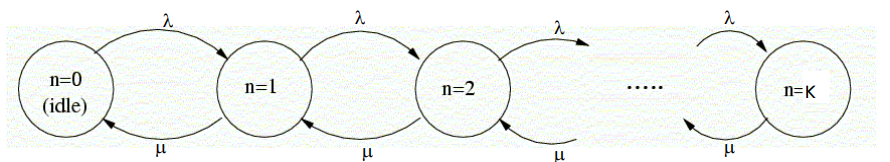
\includegraphics[width=0.8\linewidth]{figures/Lecture1/MM1K.png}
    \label{fig:placeholder}
\end{figure}
From birth-death process theory, for a finite buffer of size \(K\) (including the packet in service), with arrival rate \(\lambda\), service rate \(\mu\), and \(\rho = \lambda/\mu \neq 1\):

\begin{itemize}
    \item \textbf{Probability of \(i\) packets in the system} (steady state):
    \[
    \pi_i = \Pr(Q = i) = \frac{1 - \rho}{1 - \rho^{K+1}} \cdot \rho^{i}, \qquad i = 0,1,\dots,K.
    \]

    \item \textbf{Packet loss probability} (buffer full):
    \[
    P_{\text{loss}} = \pi_K = \frac{1 - \rho}{1 - \rho^{K+1}} \cdot \rho^{K}.
    \]

    \item \textbf{Average system delay} (time from arrival to departure):
    \[
    \bar{D} = \frac{1}{\lambda(1 - P_{\text{loss}})} \cdot \frac{\rho}{1 - \rho^{K+1}} \left[ \frac{1 - \rho^{K}}{1 - \rho} - K \rho^{K} \right].
    \]
\end{itemize}

\noindent
\textbf{Note:} For \(\rho = 1\), the formulas take limit forms (e.g., \(\pi_i = 1/(K+1)\)). The average delay formula accounts only for packets that are not lost.


\section*{The problem}

In a normal M/M/1 queue, the service rate \(\mu\) is constant.  
But in wireless communication, the channel quality can change over time (good or bad).  
\begin{itemize}
    \item When the channel is bad, transmission is slower (lower service rate \(\mu_1\)).
    \item When the channel is good, transmission is faster (higher service rate \(\mu_2 > \mu_1\)).
\end{itemize}
So the service rate depends on the \textbf{channel state} (Good or Poor).

\section*{How we model it}

We can model this as a \textbf{two-dimensional Markov chain}:

\begin{itemize}
    \item \textbf{Dimension 1}: Queue length \(n = 0, 1, 2, \dots\) (same as before).
    \item \textbf{Dimension 2}: Channel state = \(G\) (Good) or \(P\) (Poor).
\end{itemize}

So the state is a pair: \((n, G)\) or \((n, P)\).

\noindent
\textbf{Example}: \((3, P)\) means 3 packets in the system and the channel is in Poor condition.

\section*{Transition behavior – two cases}

The slide mentions two different cases for how the channel state changes:

\begin{enumerate}
    \item \textbf{Channel changes only after a successful transmission} – meaning the channel state can only change when a packet finishes service (i.e., at departure instants).\\
    \textbf{Basically} The state of the channel is only known from the description of the departure: when a packet departs, we observe whether the channel was in Poor or Good state.
    
    \item Channel may change at any moment in time (independently of service completions).
\end{enumerate}

The first case is simpler to analyze because channel transitions are synchronized with departures.

\section{Two-dimensional Markov chain structure}
\begin{figure}[H]
    \centering
    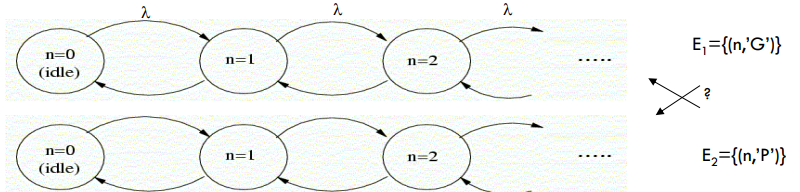
\includegraphics[width=0.9\linewidth]{figures/Lecture1/goodBad.png}
    \label{fig:placeholder}
\end{figure}
The state space is:
\[
\mathbb{E} = \{0,1,2,\dots\} \times \{G, P\}.
\]

Transitions (rates) include:
\begin{itemize}
    \item \textbf{Arrivals}: \((n, G) \to (n+1, G)\) at rate \(\lambda\); similarly for \(P\).
    \item \textbf{Departures (service)}: 
        \begin{itemize}
            \item \((n, G) \to (n-1, G)\) at rate \(\mu_2\) (good channel)
            \item \((n, P) \to (n-1, P)\) at rate \(\mu_1\) (poor channel)
        \end{itemize}
    \item \textbf{Channel state changes} (if allowed at any time): 
        \begin{itemize}
            \item \((n, G) \to (n, P)\) at some rate \(\alpha\)
            \item \((n, P) \to (n, G)\) at some rate \(\beta\)
        \end{itemize}
\end{itemize}

\section*{Solution approaches}

Because the state space is two-dimensional, simple closed-form solutions like the birth-death product formula do not apply. The slide lists two common approaches:

\begin{itemize}
    \item \textbf{Truncate and compute numerically}: Limit the maximum queue length to some \(N\) (e.g., \(N = 100\)), then solve the finite Markov chain using linear algebra.
    \item \textbf{Quasi-Birth-Death (QBD) process}: A matrix-analytic method that exploits the repeating structure of the chain (levels correspond to queue length, phases correspond to channel state).
\end{itemize}


\section{Why ON/OFF models?}

The Poisson (M/M/1) model assumes packet arrivals happen completely randomly at a constant average rate.  
But real traffic (e.g., web browsing, video streaming, sensor bursts) is \textbf{bursty} – it has periods of high activity (ON) and periods of silence (OFF).

An ON/OFF model captures this burstiness.

\section*{How it works}

Each traffic source alternates between two states:
\begin{itemize}
    \item \textbf{ON state}: source generates packets at a peak rate \(\lambda_p\) (high speed).
    \item \textbf{OFF state}: source generates no packets.
\end{itemize}
The durations of ON and OFF periods are random (often exponentially distributed).

\section*{Parameters (as in slide 43)}
\begin{figure}[H]
    \centering
    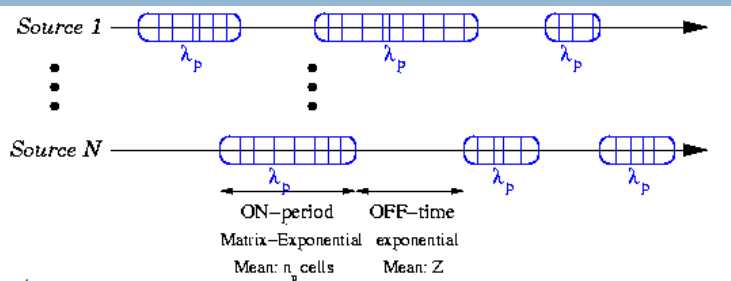
\includegraphics[width=0.8\linewidth]{figures/Lecture1/OnOff.png}
    \label{fig:placeholder}
\end{figure}
\begin{itemize}
    \item \(N\) = number of independent ON/OFF sources.
    \item Average rate per source = \(\kappa\) (long-term average throughput).
    \item Peak rate when ON = \(\lambda_p\) (much larger than \(\kappa\)).
    \item Mean ON duration and mean OFF duration are given (e.g., measured from real traffic).
\end{itemize}

The relation is:
\[
\kappa = \lambda_p \cdot \frac{\text{ON}}{\text{ON} + \text{OFF}}
\]
where ON and OFF are the \textbf{mean durations}.

\paragraph{Example:} If peak rate = 10 Mbps, ON = 0.1 sec, OFF = 0.9 sec, then average rate = \(10 \times 0.1 / 1.0 = 1\) Mbps.

\section*{Why more realistic than Poisson?}

\begin{itemize}
    \item Poisson traffic has \textbf{no memory} – the chance of a packet arriving is always the same, no matter what just happened.
    \item Real traffic often comes in \textbf{bursts} – after a packet, more packets are likely (ON period), then silence (OFF period).
    \item ON/OFF models can match the \textbf{variance and correlation} of real traffic, while Poisson only matches the average rate.
\end{itemize}

\section*{Transition rates for On/Off}

\subsection*{From state \((n, \text{ON})\):}
\begin{itemize}
    \item \textbf{Arrival (birth)}: \((n, \text{ON}) \to (n+1, \text{ON})\) at rate \(\lambda_p\) (peak rate).
    \item \textbf{Departure (death)}: if \(n \ge 1\), \((n, \text{ON}) \to (n-1, \text{ON})\) at rate \(\mu\).
    \item \textbf{Source switches to OFF}: \((n, \text{ON}) \to (n, \text{OFF})\) at rate \(\alpha\) (where \(1/\alpha\) = mean ON duration).
\end{itemize}

\subsection*{From state \((n, \text{OFF})\):}
\begin{itemize}
    \item \textbf{No arrivals} because source is silent (OFF).
    \item \textbf{Departure}: if \(n \ge 1\), \((n, \text{OFF}) \to (n-1, \text{OFF})\) at rate \(\mu\).
    \item \textbf{Source switches to ON}: \((n, \text{OFF}) \to (n, \text{ON})\) at rate \(\beta\) (where \(1/\beta\) = mean OFF duration).
\end{itemize}

\noindent
\textbf{Note:} 
\begin{itemize}
    \item When \(n = 0\) and source is OFF, the system is idle.
    \item When \(n = 0\) and source is ON, the server is idle but the source is ready to send (so the next arrival will happen at rate \(\lambda_p\)).
\end{itemize}

\section*{Why is this more complex than M/M/1?}

\begin{itemize}
    \item In M/M/1, the Markov chain is one-dimensional (just queue length).
    \item Here, the arrival rate depends on the source state, which changes randomly.
    \item The chain is \textbf{two-dimensional}, so we cannot use the simple birth-death product formula.
\end{itemize}

\section*{Solution approaches (as listed on slide)}

\begin{itemize}
    \item \textbf{Truncation}: limit maximum queue length to some large \(N\), then solve the finite Markov chain numerically (e.g., using matrix algebra).
    \item \textbf{Quasi-Birth-Death (QBD) process}: a special structure where transitions only change queue length by \(+1\), \(-1\), or keep it the same, while the source state can change. QBDs can be solved using matrix-geometric methods.
\end{itemize}

\begin{mdframed}[backgroundcolor=lightgray, linewidth=0pt, innertopmargin=8pt,
innerbottommargin=8pt]
\textbf{Key Takeaway:}
A single ON/OFF source feeding an M/M/1 queue is a \textbf{2D Markov chain} (queue length \(\times\) source state), solved numerically or with QBD techniques, because the arrival rate varies with the source's ON/OFF state.
\end{mdframed}

\section*{Hieracrhy Modeling?}

Instead of using a single Markov chain or queueing model, hierarchical models break the system into \textbf{layers of abstraction}, where each level represents events happening at a different time scale.

\begin{itemize}
    \item \textbf{Finer levels (bottom)}: short time scale (microseconds to seconds) $\rightarrow$ individual packets, bursts.
    \item \textbf{Coarser levels (top)}: long time scale (minutes to hours) $\rightarrow$ sessions, applications, access periods.
\end{itemize}

\section*{Example from the diagram (5‑level model)}
\begin{figure}[H]
    \centering
    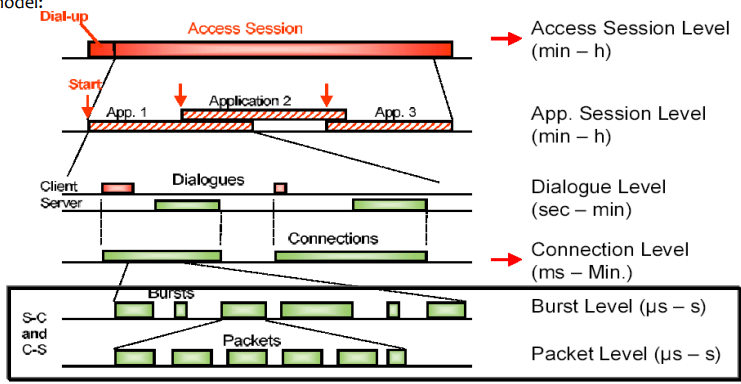
\includegraphics[width=0.9\linewidth]{figures/Lecture1/hierarchy.png}
    \caption{Caption}
    \label{fig:placeholder}
\end{figure}
\begin{table}[h!]
\centering
\caption{Five-level hierarchical model}
\begin{tabular}{>{\raggedright\arraybackslash}p{4cm} 
                >{\raggedright\arraybackslash}p{3.5cm} 
                >{\raggedright\arraybackslash}p{7cm}}
\toprule
\textbf{Level} & \textbf{Time scale} & \textbf{What it represents} \\
\midrule
Access Session Level & minutes – hours & The period a user is connected (e.g., dial‑up session, LTE attachment) \\
\hline
App. Session Level & minutes – hours & An application session (e.g., browsing session, video streaming login) \\
\hline
Dialogue Level & seconds – minutes & A conversational exchange (e.g., request‑response pairs, SIP dialogues) \\
\hline
Connection Level & milliseconds – minutes & A transport connection (e.g., TCP connection) \\
\hline
Burst Level & $\mu$s – seconds & A burst of packets (e.g., ON period in ON/OFF model) \\
\hline
Packet Level & $\mu$s – seconds & Individual packet arrivals/departures \\
\bottomrule
\end{tabular}
\end{table}

\section*{Why use hierarchical models?}

\begin{itemize}
    \item \textbf{Efficiency}: Analyzing everything at the packet level for long sessions is computationally expensive. Instead, you can model the higher levels as driving processes that generate lower‑level events with aggregated parameters.
    \item \textbf{Realism}: Network traffic naturally exhibits multiple time scales (e.g., a TCP connection consists of many bursts, which consist of many packets).
    \item \textbf{Analytical tractability}: You can use different stochastic models at each level (e.g., Markov chains for sessions, ON/OFF for bursts, M/M/1 for packets) and combine them.
\end{itemize}